\documentclass[17pt,aspectratio=169]{beamer}

\mode<presentation>
{
  \usetheme{default}
  \usecolortheme{default}
  \usefonttheme{default}
  \setbeamertemplate{navigation symbols}{}
  \setbeamertemplate{caption}[numbered]
}

\usepackage[english]{babel}
\usepackage[utf8x]{inputenc}
\usepackage{ulem}
\usepackage{booktabs}
\usepackage{adjustbox}
\usepackage{graphicx}
\usepackage{tikz}
\usetikzlibrary{shapes.geometric, arrows.meta, positioning}

% --- override footline AFTER theme is loaded ---
\makeatletter
\setbeamertemplate{footline}{
  \leavevmode%
  \hfill
  \usebeamercolor[fg]{page number in head/foot}%
  \usebeamerfont{page number in head/foot}%
  \insertframenumber{} / \inserttotalframenumber\hspace*{0.2cm}
  \vskip5pt
}
\setbeamercolor{page number in head/foot}{fg=gray}
\makeatother

\title[Your Short Title]{Explainable AI Code Generation Assistant}
\author{Author: Iuliia Liutova
\\ Supervisor: Alexander Avdiushenko}
\institute{Neapolis University Paphos}
\date{}

\begin{document}

\begin{frame}
  \titlepage
\end{frame}

\begin{frame}{Problem}
\setlength{\columnsep}{0pt}
\begin{columns}[T,totalwidth=\textwidth]

\begin{column}{0.4\textwidth}
\begin{itemize}
  \item LLMs write code, but do not explain decisions clearly.
  \item No mapping between summary and code.
\end{itemize}
\end{column}

\begin{column}{0.6\textwidth}
\vspace{-0.9cm}
\begin{figure}
    \centering
    \hspace*{0.02\linewidth}
\includegraphics[width=1.04\linewidth]{problem.png}
\end{figure}
\end{column}

\end{columns}
\end{frame}

\begin{frame}{Goal}
% Многие модели пишут код но разобраться в нем нет возможности потому что  либо огромные md как делает курсор либо парочку булет пойнтов которые непонятно к чему отностяся
Build a code assistant that \textbf{generates code and human-friendly explanations} aligned with the code.
\vspace{0.3cm} % (не обязательно, но красиво)

\centering
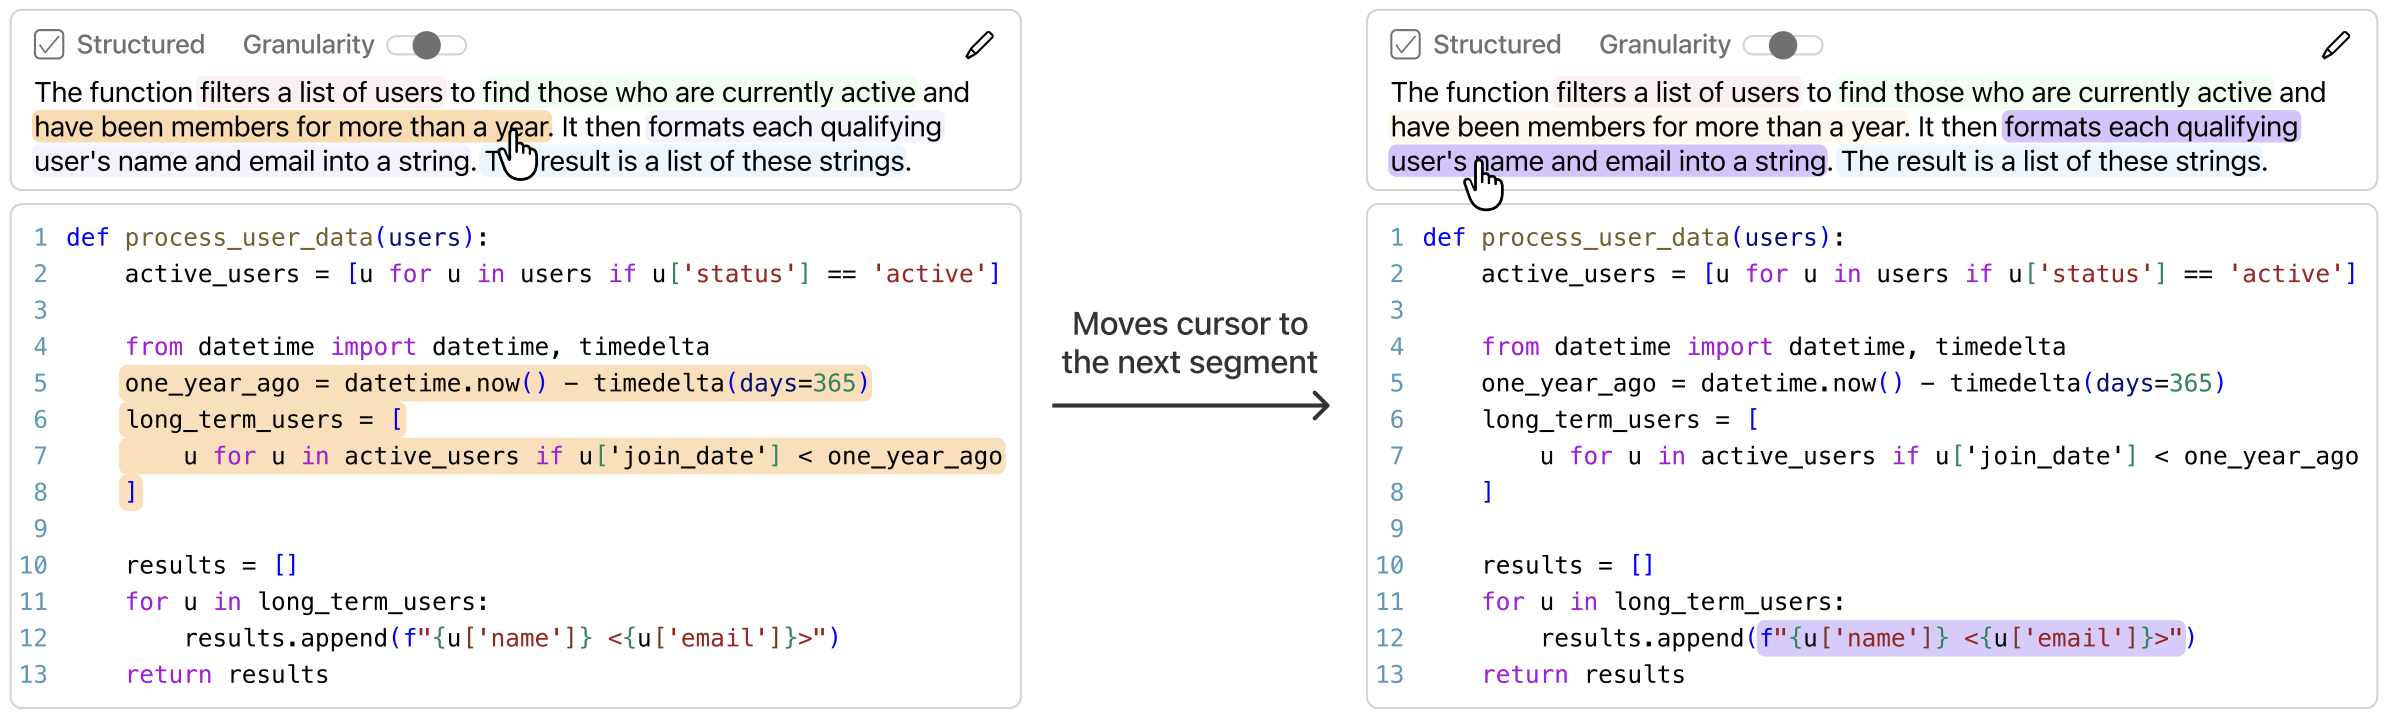
\includegraphics[width=\linewidth]{goal.png}

\end{frame}

% \begin{frame}{NaturalEdit, October 2025}
% \begin{figure}
%     \centering
%     \includegraphics[width=0.8\linewidth]{ref.png}
%     \label{fig:placeholder}
% \end{figure}
% \end{frame}

% \begin{frame}{High-level architecture}
% \begin{figure}[h]
% \centering
% \scriptsize
% \begin{tikzpicture}[
%     node distance=6mm and 8mm,
%     >=Latex,
%     every node/.style={align=center},
%     process/.style={draw, rounded corners, rectangle, minimum width=2.2cm, minimum height=7mm},
%     data/.style={draw, trapezium, trapezium left angle=75, trapezium right angle=105, minimum width=2.2cm, minimum height=7mm},
%     store/.style={draw, cylinder, shape border rotate=90, aspect=0.25, minimum height=7mm, minimum width=1.6cm},
%     decision/.style={draw, diamond, aspect=1.6, inner sep=1pt},
%     line/.style={->, thick}
% ]

% % Row 1
% \node[data] (task) {Task};
% \node[process, right=of task] (agent) {Coding AI\\Agent};
% \node[store, right=of agent] (newrepo) {New Repo};
% \node[data, right=of newrepo] (snapnew) {Snapshot of\\New Repo};

% % Row 2
% \node[store, below=12mm of task] (repo) {Repo};
% \node[data, right=of repo] (snaprepo) {Snapshot of\\Repo};
% \node[decision, right=18mm of snaprepo] (diff) {Diff};
% \node[process, right=18mm of diff] (explain) {GPT Explanation\\ / Summary};

% % Row 3
% \node[process, below=12mm of diff] (mapping) {Mapping};
% \node[process, left=of mapping] (code) {Code};
% \node[store, left=of code] (dataset) {Reference\\Dataset};
% \node[process, right=of mapping] (highlight) {Highlight\\Changes};
% \node[process, right=of highlight] (summary) {Show\\Summary};

% % Row 4
% \node[process, below=12mm of mapping] (pairs) {Pairs};
% \node[process, below=of pairs] (eval) {Evaluation};

% % Arrows
% \draw[line] (task) -- (agent);
% \draw[line] (agent) -- (newrepo);
% \draw[line] (newrepo) -- (snapnew);

% \draw[line] (repo) -- (snaprepo);
% \draw[line] (snaprepo) -- (diff);
% \draw[line] (snapnew) |- (diff);

% \draw[line] (diff) -- (explain);
% \draw[line] (explain) |- (mapping);

% \draw[line] (diff) |- (code);
% \draw[line] (dataset) -- (code);

% \draw[line] (mapping) -- (highlight);
% \draw[line] (mapping) -- (summary);
% \draw[line] (mapping) -- (pairs);
% \draw[line] (pairs) -- (eval);
% \draw[line] (dataset) |- (eval);

% \end{tikzpicture}
% \end{figure}
% \end{frame}

\begin{frame}{High-level architecture}
\centering
\vspace{0.5cm}
\resizebox{1.32\linewidth}{!}{%
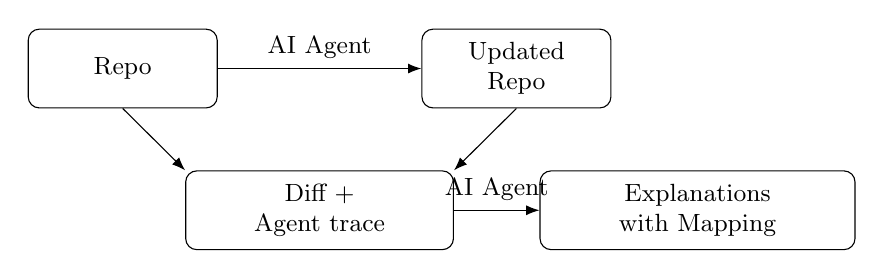
\begin{tikzpicture}[
    >=Latex,
    every node/.style={font=\small, align=center},
    block/.style={draw, rounded corners, minimum width=2.4cm, minimum height=1.0cm},
    line/.style={->, thin}
]

% Nodes
\node[block] (repo) at (0,3) {Repo};
\node[block] (updatedrepo) at (5,3) {Updated\\Repo};

\node[block, minimum width=3.4cm] (diff) at (2.5,1.2) {Diff +\\Agent trace};
\node[block, minimum width=4.0cm] (explanationmapping) at (7.3,1.2) {Explanations\\with Mapping};

% Arrows
\draw[line] (repo.east) -- node[above] {AI Agent} (updatedrepo.west);

\draw[line] (repo.south) -- (diff.north west);
\draw[line] (updatedrepo.south) -- (diff.north east);

\draw[line] (diff.east) -- node[above] {AI Agent} (explanationmapping.west);

\end{tikzpicture}%
}
\end{frame}

\begin{frame}{Code with Explanations}
\centering
\ifdefined\HCode
% HTML build (e.g., via make4ht): render an inline video player.
\HCode{<video controls preload="metadata" style="width:100%; max-width:2200px; max-height:95vh; border-radius:12px; box-shadow:0 8px 24px rgba(0,0,0,.18);"><source src="video_demo.mp4" type="video/mp4">Your browser does not support the video tag.</video>}
\else
% PDF build fallback.
\Large Video demo is available in \texttt{video\_demo.mp4}

\vspace{0.4cm}
\normalsize Open the exported HTML on GitHub Pages to play it inline.
\fi
\end{frame}

\begin{frame}[t]{Summary}
\raggedright
Done:
\begin{enumerate}
    \item Plugin prototype
    \item Initial evaluation
\end{enumerate}
Future steps:
\begin{enumerate}
    \item Experiment with using agents for explanations
    \item Extend the dataset with more diverse domains
    \item Add support for other agents
\end{enumerate}
\end{frame}

% \begin{frame}{Done work till now}
% \begin{enumerate}
%     \item Explored open source plugin for VS Code NaturalEdit
%     \item Initialization of the plugin and adding API Keys
%     \item Summary of selected code with the possibility to choose structure and granularity
%     \item Mapping and highlighting
%     \item Code generation using Junie
%     \item Catching diff
%     \item Summary with highlighting of diff
%     \item Dataset preparing
%     \item First evaluation
% \end{enumerate}
% \end{frame}

\end{document}
